\documentclass{article}
\usepackage{tikz}

\begin{document}
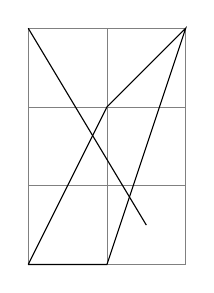
\begin{tikzpicture}
\draw[help lines] (0,0) grid (2,3);
\draw (0,0) -- (1,2)--(2,3)--(1,0)--(0,0);\draw (0,3) -- (1.5,0.5);
\end{tikzpicture}
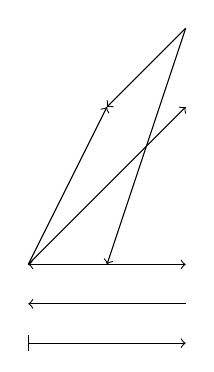
\begin{tikzpicture}
%\draw[help lines] (0,0) grid (2,3);
\draw [->] (0,0) --(2,2);
\draw [->](0,0) -- (1,2);
\draw [<-](1,2) --(2,3);
\draw [->](2,3)--(1,0);
\draw [->](1,0)--(0,0);
\draw [->] (0,0) -- (2,0);
\draw [<-] (0, -0.5) -- (2,-0.5);
\draw [|->] (0,-1) -- (2,-1);
\end{tikzpicture}
\begin{tikzpicture}
\draw [<->] (0,2) -- (0,0) -- (3,0);
\end{tikzpicture}


\begin{tikzpicture}
\draw [ultra thick] (0,1) -- (2,1);
\draw [thick] (0,0.5) -- (2,0.5);
\draw [thin] (0,0) -- (2,0);
\end{tikzpicture}

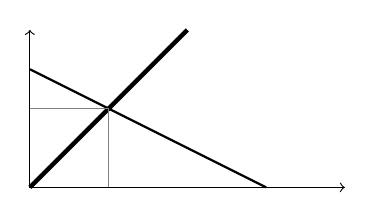
\begin{tikzpicture}
\draw [<->] (0,2) -- (0,0) -- (4,0);
\draw [thick] (0,1.5) -- (3,0);
\draw [ultra thick] (0,0) -- (2,2);
\draw [help lines] (1,0) -- (1,1) -- (0,1);
\end{tikzpicture}


\begin{tikzpicture}
\draw [line width=12] (0,0) -- (2,0);
\draw [line width=0.2cm] (4,.75) -- (5,.25);
\end{tikzpicture}

\begin{tikzpicture}
\draw [dashed, ultra thick] (0,1) -- (2,1);
\draw [dashed] (0, 0.5) -- (2,0.5);
\draw [dotted] (0,0) -- (2,0);
\end{tikzpicture}

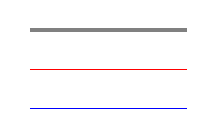
\begin{tikzpicture} 
\draw [gray, ultra thick] (0,1) -- (2,1); 
\draw [red] (0, 0.5) -- (2,0.5); 
\draw [blue] (0,0) -- (2,0); 
\end{tikzpicture}

wherever 
\begin{tikzpicture} \draw [yellow, line width=6]
(0,0) -- (.5,0);  \end{tikzpicture} you want

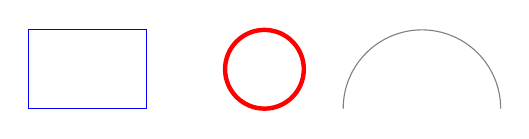
\begin{tikzpicture}
\draw [blue] (0,0) rectangle (1.5,1);
\draw [red, ultra thick] (3, 0.5) circle [radius=0.5];
\draw [gray] (6,0) arc [radius=1,start angle=0, end angle=180];
\end{tikzpicture}

\begin{tikzpicture}
\draw [<->, rounded corners, thick, purple] (0,2) -- (0,0) -- (3,0);
\end{tikzpicture}

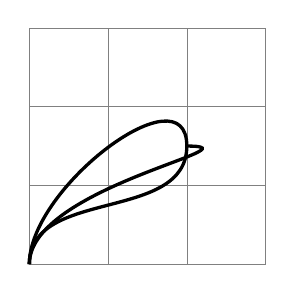
\begin{tikzpicture}
\draw[help lines] (0,0) grid (3,3);
%\draw[very thick] (0,0) to [out=90,in=360] (2,1.5);
\draw[very thick] (0,0) to [out=90,in=0] (2,1.5);
\draw[very thick] (0,0) to [out=90,in=90] (2,1.5);
\draw[very thick] (0,0) to [out=90,in=270] (2,1.5);
\end{tikzpicture}

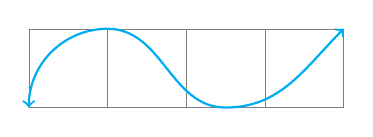
\begin{tikzpicture}
\draw[help lines] (0,0) grid (4,1);
\draw [<->,thick, cyan] (0,0) to [out=90,in=180] (1,1)
to [out=0,in=180] (2.5,0) to [out=0,in=-135] (4,1) ;
\end{tikzpicture}

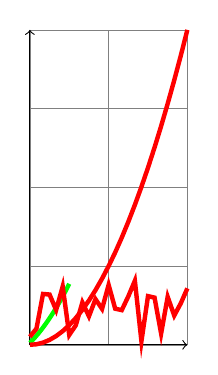
\begin{tikzpicture}
\draw[help lines] (0,0) grid (2,4);
\draw [<->] (0,4)--(0,0)--(2,0);
\draw [green,ultra thick, domain=0:0.5] plot(\x,{0.025+\x+\x*\x});
\draw [red,ultra thick, domain=0:2] plot(\x,{\x*\x});
\draw [red,ultra thick, domain=0:2] plot(\x,{rnd});
\end{tikzpicture}

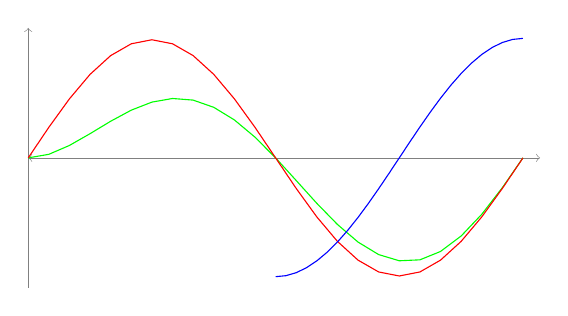
\begin{tikzpicture}[yscale=1.5]
\draw [help lines, <->]  (0,0) -- (6.5,0);
\draw [help lines, ->] (0,-1.1) -- (0,1.1);
\draw [green,domain=0:2*pi] plot (\x, {(sin(\x r)* ln(\x+1))/2});
\draw [red,domain=0:2*pi] plot (\x, {sin(\x r)});
\draw [blue, domain=pi:2*pi] plot (\x, {cos(\x r)*exp(\x/exp(2*pi))});
\end{tikzpicture}

\end{document}